\documentclass[12pt,utf8,notheorems,compress,t]{beamer}
\usepackage{etex}

\usepackage[english]{babel}

\usepackage{mathtools}
\usepackage{booktabs}
\usepackage{stmaryrd}
\usepackage{array}
\usepackage{ragged2e}
\usepackage{multicol}
\usepackage{tabto}
\usepackage{xstring}
\usepackage{ifthen}
\usepackage{soul}\setul{0.3ex}{}
\usepackage[all]{xy}
\xyoption{rotate}
\usepackage{tikz}
\usetikzlibrary{mindmap,calc,shapes,shapes.callouts,shapes.arrows,patterns,fit,backgrounds,decorations.pathmorphing}
\hypersetup{colorlinks=false}

\usepackage{pifont}
\newcommand{\cmark}{\ding{51}}
\newcommand{\xmark}{\ding{55}}

\graphicspath{{images/}}

\usepackage[protrusion=true,expansion=true]{microtype}

\setlength\parskip{\medskipamount}
\setlength\parindent{0pt}

\title{How topos theory can help algebra and geometry}
\author{Ingo Blechschmidt}
\date{July 10th, 2018}

\useinnertheme[shadow=true]{rounded}
\useoutertheme[subsection=false]{miniframes}
\setbeamerfont{block title}{size={}}

\useinnertheme{rectangles}

\usecolortheme{orchid}
\usecolortheme{seahorse}
\definecolor{mypurple}{RGB}{150,0,255}
\setbeamercolor{structure}{fg=mypurple}
\definecolor{myred}{RGB}{150,0,0}
\setbeamercolor*{title}{bg=myred,fg=white}
\setbeamercolor*{titlelike}{bg=myred,fg=white}
\setbeamercolor{frame}{bg=black}

\usefonttheme{serif}
\usepackage[T1]{fontenc}
\usepackage{libertine}

\newcommand{\A}{\mathcal{A}}
\newcommand{\B}{\mathcal{B}}
\renewcommand{\AA}{\mathbb{A}}
\renewcommand{\C}{\mathcal{C}}
\newcommand{\E}{\mathcal{E}}
\newcommand{\F}{\mathcal{F}}
\newcommand{\M}{\mathcal{M}}
\renewcommand{\G}{\mathcal{G}}
\newcommand{\J}{\mathcal{J}}
\newcommand{\GG}{\mathbb{G}}
\renewcommand{\O}{\mathcal{O}}
\newcommand{\K}{\mathcal{K}}
\newcommand{\NN}{\mathbb{N}}
\newcommand{\QQ}{\mathbb{Q}}
\newcommand{\RR}{\mathbb{R}}
\newcommand{\TT}{\mathbb{T}}
\newcommand{\PP}{\mathbb{P}}
\newcommand{\ZZ}{\mathbb{Z}}
\renewcommand{\P}{\mathcal{P}}
\newcommand{\aaa}{\mathfrak{a}}
\newcommand{\fff}{\mathfrak{f}}
\newcommand{\ppp}{\mathfrak{p}}
\newcommand{\mmm}{\mathfrak{m}}
\newcommand{\defeq}{\vcentcolon=}
\newcommand{\defeqv}{\vcentcolon\equiv}
\newcommand{\Sh}{\mathrm{Sh}}
\newcommand{\GL}{\mathrm{GL}}
\newcommand{\Zar}{\mathrm{Zar}}
\newcommand{\op}{\mathrm{op}}
\newcommand{\Set}{\mathrm{Set}}
\newcommand{\Ring}{\mathrm{Ring}}
\newcommand{\LocRing}{\mathrm{LocRing}}
\newcommand{\Eff}{\mathrm{Ef{}f}}
\newcommand{\Sch}{\mathrm{Sch}}
\newcommand{\Aff}{\mathrm{Aff}}
\newcommand{\LRS}{\mathrm{LRS}}
\newcommand{\Hom}{\mathrm{Hom}}
\newcommand{\Spec}{\mathrm{Spec}}
\newcommand{\lra}{\longrightarrow}
\newcommand{\RelSpec}{\operatorname{Spec}}
\renewcommand{\_}{\mathpunct{.}}
\newcommand{\?}{\,{:}\,}
\newcommand{\speak}[1]{\ulcorner\text{\textnormal{#1}}\urcorner}
\newcommand{\ull}[1]{\underline{#1}}
\newcommand{\affl}{\ensuremath{{\ull{\AA}^1}}}
\newcommand{\Ll}{\text{iff}}
\newcommand{\inv}{inv.\@}
\newcommand{\seq}{\vdash_{\!\!\!\vec x}}
\newcommand{\hg}{\mathbin{:}}  % homogeneous coordinates

\setbeamertemplate{blocks}[rounded][shadow=false]

% Adapted from https://latex.org/forum/viewtopic.php?t=2251 (Stefan Kottwitz)
\newenvironment<>{hilblock}{
  \begin{center}
    \begin{minipage}{9.05cm}
      \setlength{\textwidth}{9.05cm}
      \begin{actionenv}#1
        \def\insertblocktitle{}
        \par
        \usebeamertemplate{block begin}}{
        \par
        \usebeamertemplate{block end}
      \end{actionenv}
    \end{minipage}
  \end{center}}

\newcommand{\bignumber}[1]{
  \renewcommand{\insertenumlabel}{#1}\scalebox{1.5}{\usebeamertemplate{enumerate item}}
}

\newenvironment{indentblock}{%
  \list{}{\leftmargin\leftmargin}%
  \item\relax
}{%
  \endlist
}

\newcommand{\hcancel}[5]{%
  \tikz[baseline=(tocancel.base)]{
    \node[inner sep=0pt,outer sep=0pt] (tocancel) {#1};
    \draw[red, line width=0.4mm] ($(tocancel.south west)+(#2,#3)$) -- ($(tocancel.north east)+(#4,#5)$);
  }%
}

\newenvironment{changemargin}[2]{%
  \begin{list}{}{%
    \setlength{\topsep}{0pt}%
    \setlength{\leftmargin}{#1}%
    \setlength{\rightmargin}{#2}%
    \setlength{\listparindent}{\parindent}%
    \setlength{\itemindent}{\parindent}%
    \setlength{\parsep}{\parskip}%
  }%
  \item[]}{\end{list}}

\tikzset{
  invisible/.style={opacity=0,text opacity=0},
  visible on/.style={alt={#1{}{invisible}}},
  alt/.code args={<#1>#2#3}{%
    \alt<#1>{\pgfkeysalso{#2}}{\pgfkeysalso{#3}}}
}

\newcommand{\pointthis}[3]{%
  \tikz[remember picture,baseline]{
    \node[anchor=base,inner sep=0,outer sep=0] (#2) {#2};
    \node[visible on=#1,overlay,rectangle callout,rounded corners,callout relative pointer={(0.3cm,0.5cm)},fill=blue!20] at ($(#2.north)+(-0.1cm,-1.1cm)$) {#3};
  }%
}

% Adapted from https://latex.org/forum/viewtopic.php?t=2251 (Stefan Kottwitz)
\newenvironment<>{varblock}[2]{
  \begin{center}
    \begin{minipage}{#1}
      %\setlength{\textwidth}{#1}
      \begin{actionenv}#3
  \def\insertblocktitle{\centering #2}
  \par
  \usebeamertemplate{block begin}}{
        \par
        \usebeamertemplate{block end}
      \end{actionenv}
    \end{minipage}
  \end{center}}

\setbeamertemplate{frametitle}{%
  \vskip0.7em%
  \leavevmode%
  \begin{beamercolorbox}[dp=1ex,center]{}%
      \usebeamercolor[fg]{item}{\textbf{{\Large \insertframetitle}}}
  \end{beamercolorbox}%
}

\setbeamertemplate{navigation symbols}{}

\newcounter{framenumberpreappendix}
\newcommand{\backupstart}{
  \setcounter{framenumberpreappendix}{\value{framenumber}}
}
\newcommand{\backupend}{
  \addtocounter{framenumberpreappendix}{-\value{framenumber}}
  \addtocounter{framenumber}{\value{framenumberpreappendix}}
}

\setbeamertemplate{footline}{%
  \begin{beamercolorbox}[wd=\paperwidth,ht=2.25ex,dp=1ex,right,rightskip=1mm,leftskip=1mm]{}%
    % \inserttitle
    \hfill
    \insertframenumber\,/\,\inserttotalframenumber
  \end{beamercolorbox}%
  \vskip0pt%
}


\newcommand{\hil}[1]{{\usebeamercolor[fg]{item}{\textbf{#1}}}}

\newcommand{\bad}[1]{\textcolor{red!90}{\textnormal{#1}}}


\begin{document}

\tikzstyle{topos} = [draw=mypurple, very thick, rectangle, rounded corners, inner sep=5pt, inner ysep=10pt]
\tikzstyle{title} = [fill=mypurple, text=white]

% Taken from Todd Lehman (CC-BY-SA) at https://tex.stackexchange.com/a/44920/32372

\newcommand{\setisprime}[1]{
  % Sets \isprime based on #1.
  \ifnum#1=1 \gdef\isprime{0} \else \gdef\isprime{1} \fi
  \foreach \sip in {2, 3,5,...,#1} {
    \pgfmathparse{\sip*\sip>#1? 1:0}
    \ifthenelse{\pgfmathresult=1}{
      % Early-out if \sip^2 > #1.
      \breakforeach
    }{
      % Otherwise test if \sip divides #1.
      \pgfmathparse{Mod(#1,\sip)==0? 1:0}
      \ifthenelse{\pgfmathresult=1}{
        \gdef\isprime{0}
        \breakforeach
      }{}
    }
  }
}

\newcommand{\setxy}[1]{
  % Sets \x and \y to loction of cell #1.
  \pgfmathtruncatemacro{\x}{Mod(#1-1,\cols)}
  \pgfmathtruncatemacro{\y}{(#1-1) / \cols}
  \pgfmathtruncatemacro{\y}{\cols - 1 - \y}
  \pgfmathparse{2.5*(\x+.5)}\let\x\pgfmathresult
  \pgfmathparse{2.5*(\y+.5)}\let\y\pgfmathresult
}

\newcommand{\numlabel}[2]{
  % Draws label #2 at cell #1.
  \setxy{\n}
  \node[fill=none, text=black] at (\x,\y) {#2};
}

\newcommand{\drawpolygon}[2]{
  % Draws polygon with #2 vertexes at cell #1.
  \setxy{#1}
  \ifthenelse{#2>1}{ % Polygon must have at least 2 sides.
    \ifthenelse{#2<30}{ % Draw polygon if it has a small number of sides.
      \filldraw (\x,\y) +(90:1)
      \foreach \drawi in {1,...,#2} {-- +(\drawi/#2*360+90:1)} -- cycle;
    }{ % Else approximate with circle.
      \filldraw (\x,\y) circle(1);
    }
  }{}
}

\newcommand{\setpolygoncolor}[1]{
  % Sets color based on #1.
  \gdef\polycolor{black}
  \ifnum#1=2\gdef\polycolor{black!50!white}\fi
  \ifnum#1=3\gdef\polycolor{yellow!95!red}\fi
  \ifnum#1=5\gdef\polycolor{yellow!0!red}\fi
  \ifnum#1=7\gdef\polycolor{blue!75!green}\fi
  \ifnum#1=11\gdef\polycolor{blue!70!red}\fi
  \ifnum#1=13\gdef\polycolor{blue!40!red}\fi
  \ifnum#1=17\gdef\polycolor{green!50!blue}\fi
  \ifnum#1=19\gdef\polycolor{green!80!black}\fi
  \ifnum#1=23\gdef\polycolor{green!50!red}\fi
  \ifnum#1=29\gdef\polycolor{yellow!50!black}\fi
  \ifnum#1=31\gdef\polycolor{orange!50!black}\fi
  \ifnum#1=37\gdef\polycolor{red!50!black}\fi
  \ifnum#1=41\gdef\polycolor{purple!50!black}\fi
  \ifnum#1=43\gdef\polycolor{blue!50!black}\fi
  \ifnum#1=47\gdef\polycolor{green!50!black}\fi
  \ifnum#1=53\gdef\polycolor{white!50!black}\fi
  \ifnum#1=59\gdef\polycolor{white!50!black}\fi
  \ifnum#1=61\gdef\polycolor{white!50!black}\fi
  \ifnum#1=67\gdef\polycolor{white!50!black}\fi
}

\newcommand{\sieve}[2]{
  \def\cols{#1}
  \def\rows{#2}
  \begin{tikzpicture}[scale=.5]
  \pgfmathtruncatemacro{\nmax}{\rows * \cols}

  \foreach \n in {1,...,\nmax} {
    \begin{scope}[fill=gray, fill opacity=.05,
                  draw=gray, draw opacity=.10,
                  line width=4]
      \drawpolygon{\n}{\n}
    \end{scope}
    \setisprime{\n}
    \ifthenelse{\isprime=1}{
      \numlabel{\n}{\bf\n}
    }{
      \def\startintensity{.33}
      \def\incrintensity{.10}
      \def\intensity{\startintensity}

      \def\m{\n}
      \pgfmathtruncatemacro{\i}{\m / 2}

      % Divide \m by \i until \m is extinguished.
      % Increment \i each time it does not divide into \m.
      \whiledo{\m>1}{
        \setisprime{\i}
        \pgfmathparse{Mod(\m,\i)==0? 1:0}
        \ifthenelse{\pgfmathresult=1\and\isprime=1}{
          \setpolygoncolor{\i}
          \begin{scope}[fill=\polycolor, fill opacity=\intensity,
                        draw=\polycolor!85!black, draw opacity=\intensity,
                        line width=\intensity*1.5]
            \drawpolygon{\n}{\i}
          \end{scope}
          \pgfmathtruncatemacro{\m}{\m / \i}
          \pgfmathparse{\intensity + \incrintensity}\let\intensity\pgfmathresult
        }{
          \pgfmathtruncatemacro{\i}{\i - 1}
          \def\intensity{\startintensity}
        }
      }
      \begin{scope}[text=black, text opacity=.5]
        \numlabel{\n}{\scriptsize\n}
      \end{scope}
    }
  }

  \end{tikzpicture}
}

%\renewcommand{\sieve}[2]{SIEVE}
%\renewcommand{\fakesieve}[2]{SIEVE}

\newcommand{\drawbox}[4]{
  \node[topos, #4] [fit = #3] (#1) {};
  \node[title] at (#1.north) {#2};
}

\newcommand{\muchstuff}{
  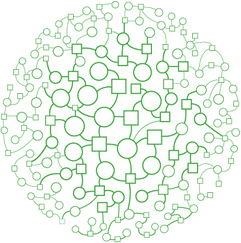
\includegraphics[height=3em]{filmat}
  \scalebox{0.5}{\sieve{14}{2}}
}

\newcommand{\muchstuffplaceholder}{
  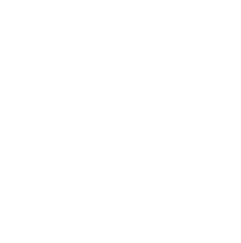
\includegraphics[height=3em]{filmat-placeholder}
  \scalebox{0.5}{\fakesieve{14}{2}}
}

\newcommand{\fewstuff}{
  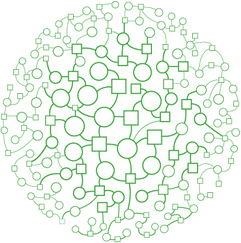
\includegraphics[height=3em]{filmat}
  \scalebox{0.5}{\sieve{7}{2}}
}

\newcommand{\threeblobs}{
  \colorbox{mypurple}{\ \ }\quad
  \colorbox{mypurple}{\ \ }\quad
  \colorbox{mypurple}{\ \ }
}

\addtocounter{framenumber}{-1}

{\usebackgroundtemplate{\begin{minipage}{\paperwidth}\vspace*{4.95cm}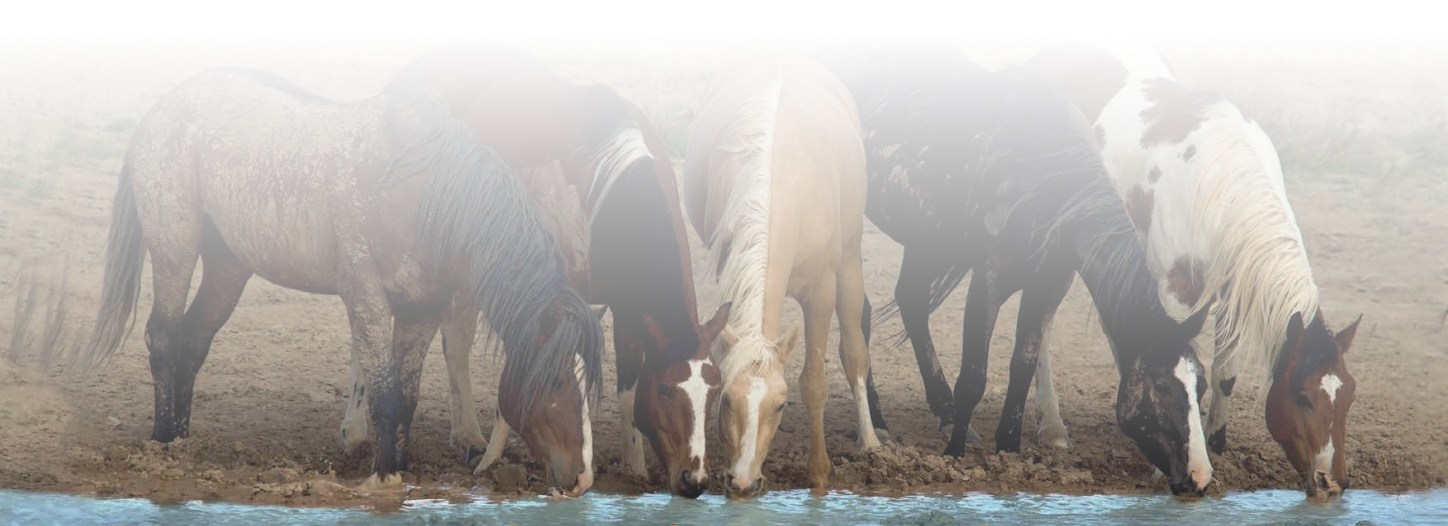
\includegraphics[width=\paperwidth]{topos-horses}\end{minipage}}
\begin{frame}[c]
  \centering
  \medskip
  \hspace*{-3.9em}%

  \hil{How topos theory can help algebra and geometry} \\

  \emph{-- an invitation --}

  \vfill

  \scriptsize
  Ingo Blechschmidt \\
  July 10th, 2018
  \par
\end{frame}}

\begin{frame}{Toposes are \ldots}
  \begin{columns}
    \begin{column}{0.5\textwidth}
      \centering
      \hil{generalized spaces}
      \medskip

      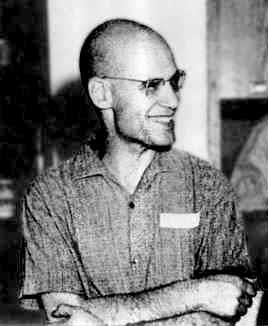
\includegraphics[height=0.35\textwidth]{grothendieck}
      \quad
      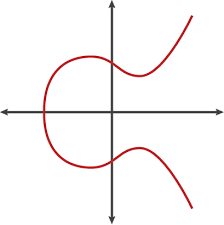
\includegraphics[height=0.35\textwidth]{elliptic-curve}

      étale topos of a scheme
    \end{column}

    \begin{column}{0.5\textwidth}
      \centering
      \hil{mathematical universes}
      \medskip

      \begin{tikzpicture}
        \node (overview) {
          \scalebox{0.32}{\sieve{6}{4}}
        };
        \def\R{8pt}
        \begin{pgfonlayer}{background}
        \draw[decoration={bumps,segment length=8pt}, decorate, very thick, draw=mypurple]
          ($(overview.south west) + (\R, 0)$) arc(270:180:\R) --
          ($(overview.north west) + (0, -\R)$) arc(180:90:\R) --
          ($(overview.north east) + (-\R, 0)$) arc(90:0:\R) --
          ($(overview.south east) + (0, \R)$) arc(0:-90:\R) --
          cycle;
        \end{pgfonlayer}
      \end{tikzpicture}
    \end{column}
  \end{columns}

  \bigskip
  \bigskip

  \begin{columns}
    \begin{column}{0.5\textwidth}
      \centering
      \hil{categories of sheaves}
      \medskip

      
\includegraphics[height=0.35\textwidth]{sheaf}

      \footnotesize
      A topos is a finitely complete cartesian closed category with a
      subobject classifier.
    \end{column}

    \begin{column}{0.5\textwidth}
      \centering
      \hil{embodiments of theories}
      \medskip

      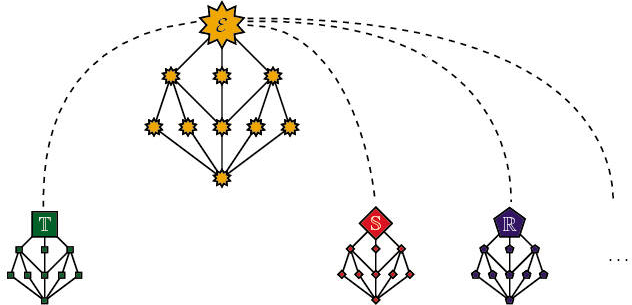
\includegraphics[height=0.35\textwidth]{olivia-lattices}

      ``Let~$G$ be a group.''
    \end{column}
  \end{columns}
\end{frame}


\section{A glimpse of the toposophic landscape}

\begin{frame}[fragile]{A glimpse of the toposophic landscape}
  \hspace*{-1em}%
  \begin{tikzpicture}
    \node (objs-set0) at (0,0) {
      \only<1-2>{\muchstuffplaceholder}
      \only<3>{\muchstuff}
    };
    \node[scale=0.4] (objs-set1) at (-4.0,-2.5) {
      \only<1->{\fewstuff}
    };
    \node[scale=0.4] (objs-eff1) at (4.0,-2.5) {
      \only<2->{\fewstuff}
    };
    \node[scale=0.4] (objs-sh1)  at (0,-2.5) {
      \only<2->{\fewstuff}
    };

    \node (prop-set1) [below of=objs-set1, align=left] {
      \only<1->{%
        The usual laws \\
        of logic hold.
      }
    };

    \node (prop-eff1) [below of=objs-eff1, align=left] {
      \only<2->{%
        Every function \\
        is computable.
      }
    };

    \node (prop-sh1) [below of=objs-sh1, align=left, inner sep=0pt] {
      \only<2->{%
        The intermediate \\
        value theorem fails.
      }
    };

    \node (more-eff1) [below of=prop-eff1, visible on=<3->] {
      \threeblobs
    };
    \node (more-sh1)  [below of=prop-sh1, visible on=<3->] {
      \threeblobs
    };
    \node (more-set1) [below of=prop-set1, visible on=<3->] {
      \threeblobs
    };

    \begin{scope}[visible on=<1->]
      \drawbox{set1}{$\mathrm{Set}$}{(objs-set1) (prop-set1) (more-set1)}{}
    \end{scope}
    \begin{scope}[visible on=<2->]
      \drawbox{eff1}{Ef{}f}{(objs-eff1) (prop-eff1) (more-eff1)}{tape}
    \end{scope}
    \begin{scope}[visible on=<2->]
      \drawbox{sh1}{$\mathrm{Sh}\, X$}{(objs-sh1) (prop-sh1) (more-sh1)}{draw=none}
      \def\R{8pt}
      \begin{pgfonlayer}{background}
      \draw[decoration={bumps,segment length=8pt}, decorate, very thick, draw=mypurple, visible on=<2->]
        ($(sh1.south west) + (\R, 0)$) arc(270:180:\R) --
        ($(sh1.north west) + (0, -\R)$) arc(180:90:\R) --
        ($(sh1.north east) + (-\R, 0)$) arc(90:0:\R) --
        ($(sh1.south east) + (0, \R)$) arc(0:-90:\R) --
        cycle;
      \end{pgfonlayer}
    \end{scope}
    \begin{scope}[visible on=<3->]
      \drawbox{set0}{$\mathrm{Set}$}{(objs-set0) (set1) (eff1) (sh1)}{}
    \end{scope}
  \end{tikzpicture}
\end{frame}


\begin{frame}{The internal universe of a topos}
  For any topos~$\E$ and any statement~$\varphi$, we define the meaning of
  \vspace*{-0.5em}
  \[
    \text{``$\E \models \varphi$''} \quad
    \text{(``$\varphi$ holds in the internal universe of~$\E$'')}
  \]

  \vspace*{-1.0em}
  using the \hil{Kripke--Joyal semantics}.

  \vspace*{-1em}
  \begin{columns}
    \def\insertblocktitle{}
    \begin{column}{0.3\textwidth}\usebeamertemplate{block begin}
      \centering
      $\Set \models \varphi$ \\
      ``$\varphi$ holds in the usual sense.''
    \usebeamertemplate{block end}\end{column}

    \begin{column}{0.3\textwidth}\usebeamertemplate{block begin}
      \centering
      $\Sh(X) \models \varphi$ \\
      ``$\varphi$ holds continuously.''
    \usebeamertemplate{block end}\end{column}

    \begin{column}{0.3\textwidth}\usebeamertemplate{block begin}
      \centering
      $\Eff \models \varphi$ \\
      ``$\varphi$ holds computably.''
    \usebeamertemplate{block end}\end{column}
  \end{columns}
  \medskip

  \pause
  Any topos supports \hil{mathematical reasoning}:

  \vspace*{-1.5em}
  \begin{hilblock}
    If~$\E \models \varphi$ and if~$\varphi \vdash \psi$
    \pointthis{<3>}{intuitionistically}{%
      no $\varphi \vee \neg\varphi$,\ \
      no $\neg\neg\varphi \Rightarrow \varphi$,\ \
      no axiom of choice},
    then~$\E \models \psi$.
  \end{hilblock}
  \bigskip
\end{frame}


\newcommand{\intex}[3]{#1 \quad #2\par #3\bigskip\medskip}

\begin{frame}{First steps in alternate universes}
  \begin{changemargin}{-1.1em}{0em}
    \fontsize{10pt}{12pt}\selectfont
    \begin{itemize}
      \item \intex{
        $\Eff \models \text{``Any number is prime or is not prime.''}$
      }{\textcolor{green!90}{\cmark}}{
        Meaning: There is a \hil{Turing machine} which determines of
        any given number whether it is prime or not.
      }

      \item \intex{
        $\Eff \models \text{``There are infinitely many prime numbers.''}$
      }{\textcolor{green!90}{\cmark}}{
        Meaning: There is a \hil{Turing machine} producing arbitrarily many
        primes.\\[0em]
      }

      \item \intex{
        $\Eff \models \text{``Any function~$\NN \to \NN$ is the zero function or not.''}$
      }{\textcolor{red!80}{\xmark}}{
        Meaning: There is a \hil{Turing machine} which, given a Turing
        machine computing a function~$f : \NN \to \NN$, determines whether~$f$
        is zero or not.
      }

      \item \intex{
        $\Eff \models \text{``Any function~$\NN \to \NN$ is computable.''}$
      }{\textcolor{green!90}{\cmark}}{}

      \item \intex{
        $\Sh(X) \models \text{``Any cont. function with opposite signs has
        a zero.''}$
      }{\textcolor{red!80}{\xmark}}{
        Meaning: Zeros can locally be picked \hil{continuously} in
        continuous families of continuous functions.
        \textcolor{red!80}{(\href{https://rawgit.com/iblech/internal-methods/master/images/zeros-in-families.mp4}{video} for counterexample)}
      }
    \end{itemize}
  \end{changemargin}
\end{frame}

\end{document}
